%\begin{figure*}[t]
%\begin{center}
%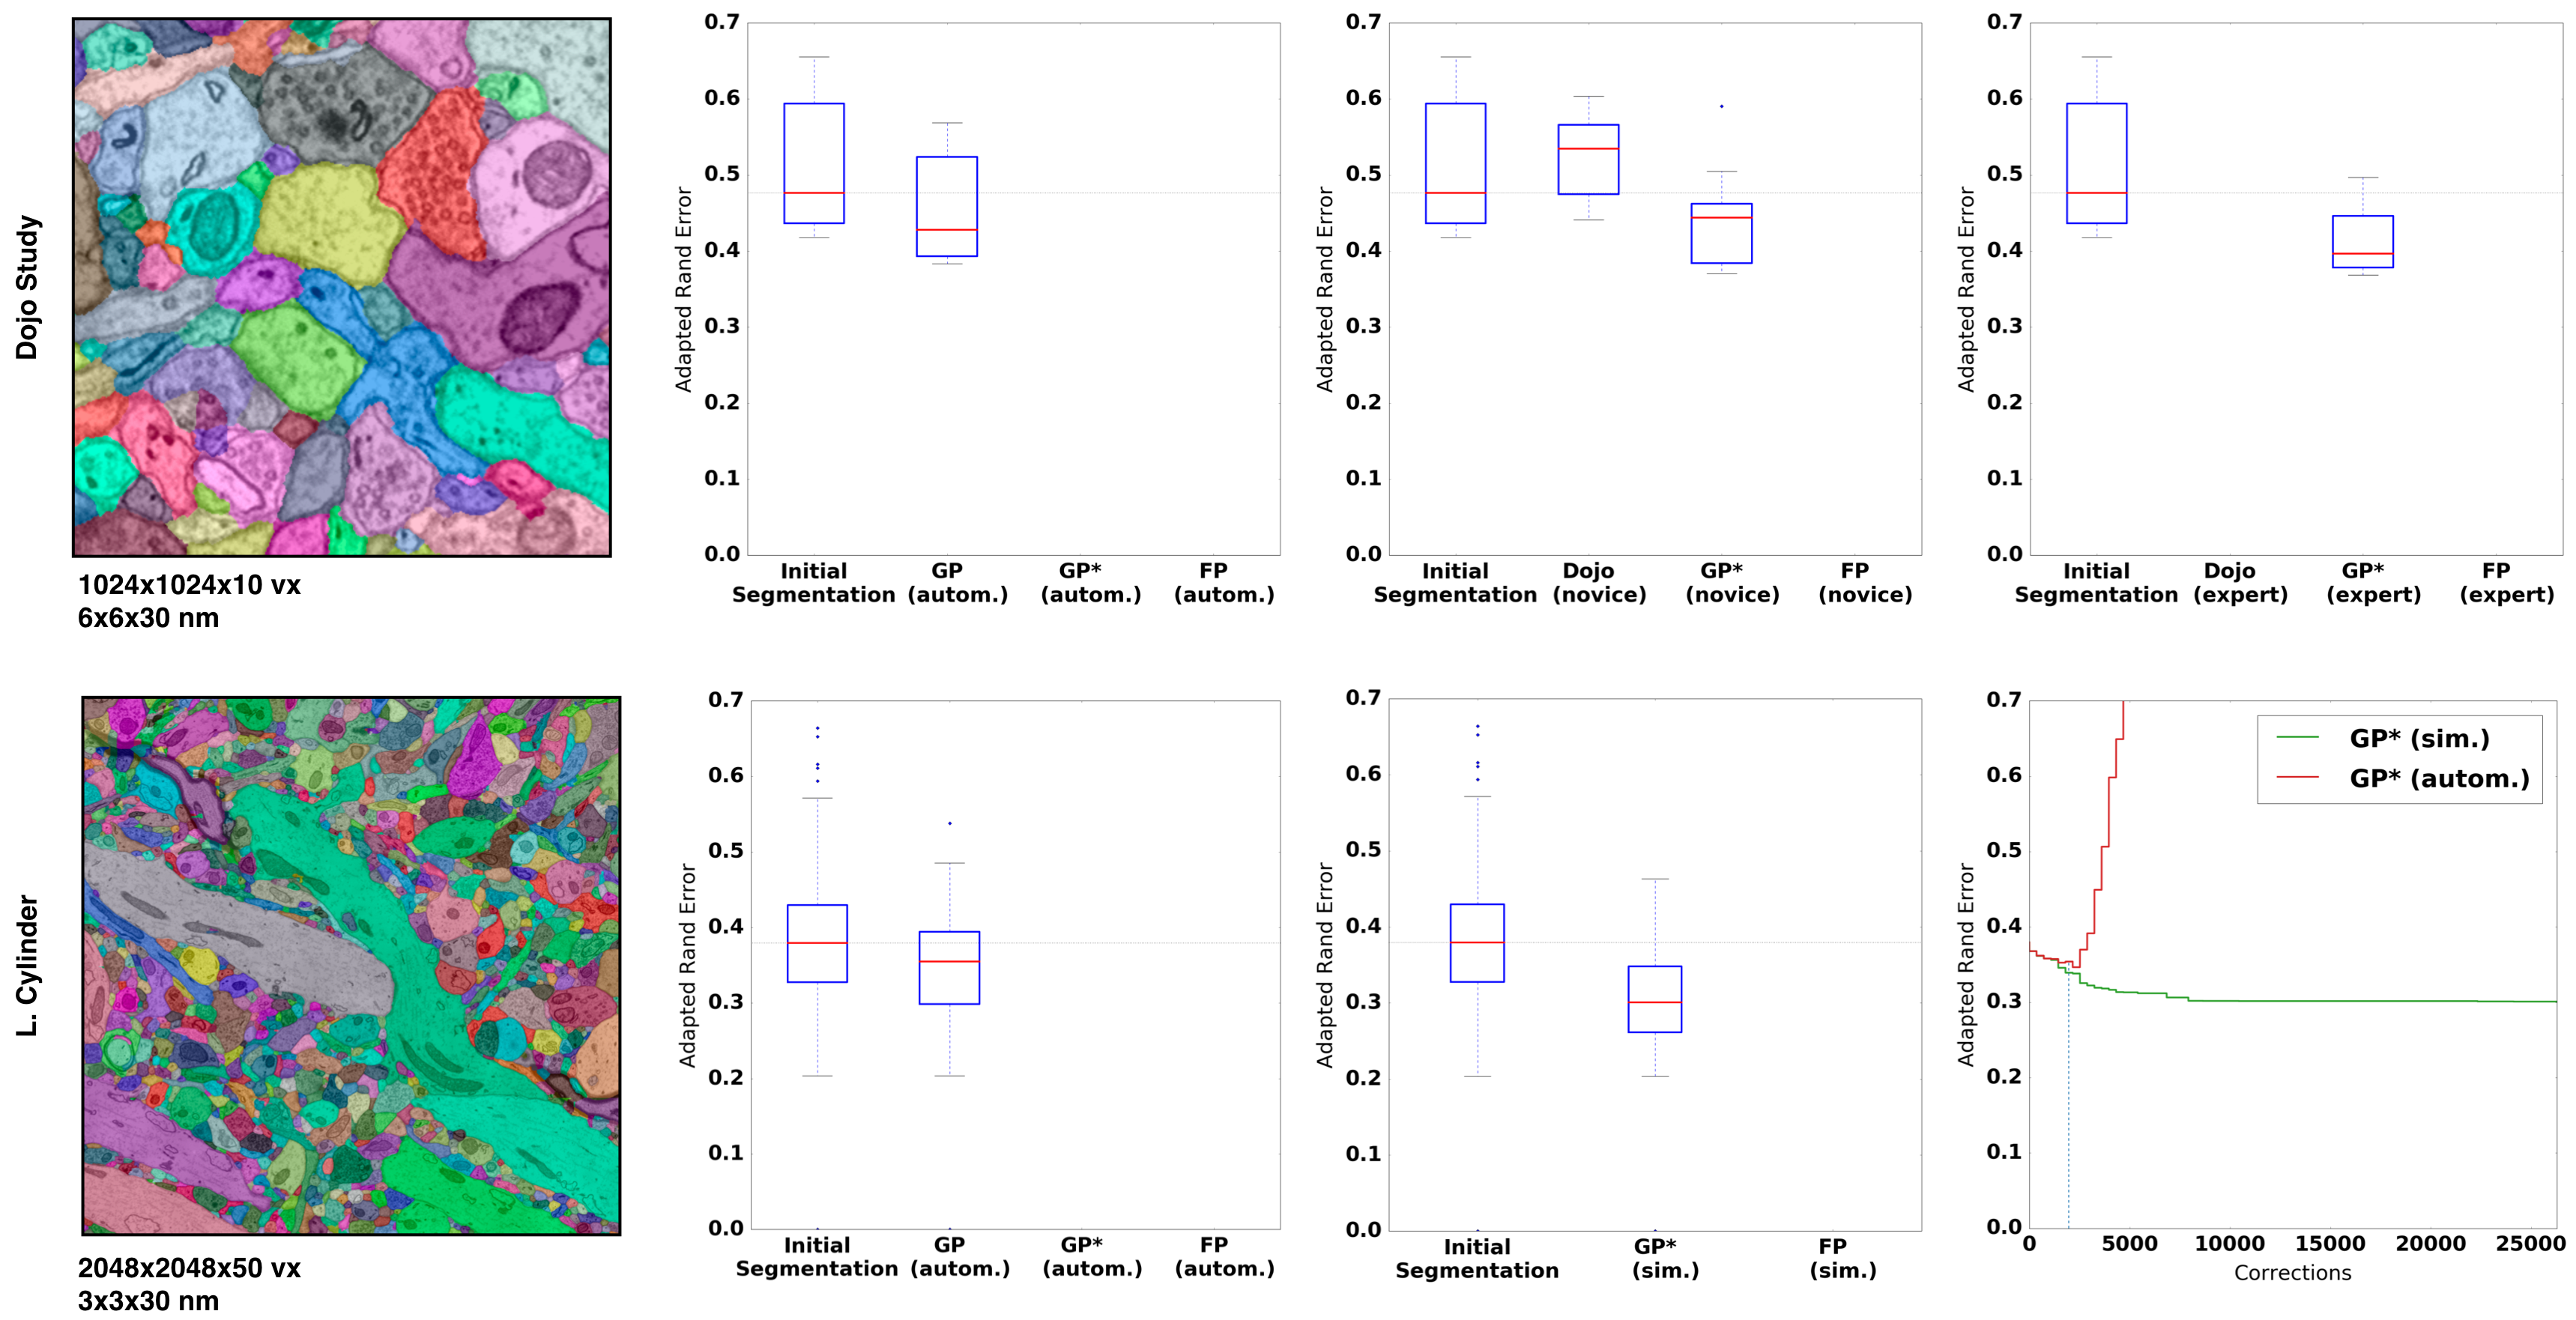
\includegraphics[width=\linewidth]{gfx/results_mouse.png}
%\end{center}
%  \vspace{-4mm}
%   \caption{Performance evaluation of the classifiers on two mouse brain datasets measured as adapted Rand error (lower scores are better). We compare guided proofreading (GP), guided proofreading with active label suggestion (GP*) and focused proofreading. Proofreading is performed automatically (autom., with probability threshold $p_t=.95$), simulated as a perfect user (sim.), or by novice and expert users as indicated. The first row of images shows the results of a user study and includes comparisons to the interactive proofreading software Dojo by Haehn \etal \cite{haehn_dojo_2014}. GP* is able to correct the segmentation further than other methods. The second row shows the results of the simulated user compared to automatic GP* and FP performance. The bottom right graph compares automatic GP* and simulated GP* per individual correction. The blue dashed line here indicates the moment the probability threshold $p_t$ is reached. The simulated user is able to correct the initial segmentation beyond this threshold while automatic GP* then introduces errors.}
%\label{fig:results_mouse}
%\end{figure*}

\section{Evaluation}
\label{sec:evaluation}

We evaluate guided proofreading on multiple different real-world connectomics datasets of different species. All datasets were acquired using either serial section electron microscopy (ssEM) or serial section transmission electron microscopy (ssTEM). We perform experiments with the selection oracle, with automatic selection with threshold, and in the forced choice setting via a between-subjects user study with both novice and expert participants.

\subsection{Datasets}

\paragraph{L. Cylinder.} We use the left part of the 3-cylinder mouse cortex volume of Kasthuri \etal~\cite{kasthuri2015saturated} ($2048\times2048\times300$ voxels). The tissue is dense mammalian neuropil from layers 4 and 5 of the S1 primary somatosensory cortex of a healthy mouse, and was acquired using ssEM. The dataset resolution is $3\times3\, \text{nm}^2$ per pixel, with section thickness of $30\, \text{nm}$. Image data and a manually-labeled expert `ground truth' segmentation is available publicly for the entire dataset\footnote{\scriptsize{\url{https://software.rc.fas.harvard.edu/lichtman/vast/}}}.

\paragraph{AC4 subvolume.} This is part of a publicly-available dataset of mouse cortex that was published for the ISBI 2013 challenge ``SNEMI3D: 3D Segmentation of neurites in EM images''. The dataset resolution is $6\times6\times30~\text{nm}^3\text{/voxel}$ and it was acquired using ssEM. Haehn~\etal~\cite{haehn_dojo_2014} found the most representative subvolume ($400\times400\times10$ voxels) of this dataset with respect to the distribution of object sizes, and used it for their interactive connectomics proofreading tool experiments. We use their publicly available data, labeled ground truth, and study findings\footnote{\scriptsize{\url{http://rhoana.org/dojo/}}}.

\paragraph{CREMI A/B/C.} As part of the MICCAI 2016 challenge on circuit reconstruction from electron microscopy images (CREMI), six ssTEM datasets were made publicly available\footnote{\scriptsize{\url{http://www.cremi.org}}},  each $1250\times1250\times125$ voxels. Since only three datasets include manually-labeled `ground truth', we use these three volumes for our experiments. The volumes are part of an adult fruit fly (Drosophila melanogaster) brain. The resolution of all three datasets is $4\times4\times40~\text{nm}^3\text{/voxel}$.

\paragraph{Automatic segmentation pipeline.}
We use a state-of-the-art method to create a dense automatic segmentation of the data. Membrane probabilities are generated using a CNN based on the U-net architecture~\cite{RonnebergerFB15}. The probabilities are used to seed watershed and generate an oversegmentation using superpixels. Agglomeration is then performed by the GALA active learning classifier~\cite{nunez2014graph}.

\subsection{Classifier Training}

We train our split error classifier on the L. Cylinder dataset. We use the first 250 sections of the data for training and validation. For n-fold cross validation, we select one quarter of this data and re-select after each epoch. We minimize cross-entropy loss and update using stochastic gradient descent with Nesterov momentum~\cite{nesterov}. To generate training data, we identify correct regions and split errors in the automatic segmentation by intersection with ground truth regions. This is required since extracellular space is not labeled in the ground truth, but is in our dense automatic segmentation. From these regions, we sample 112,760 correct and 112,760 split error patches with 4-channels (Sec.~\ref{sec:spliterrordetection}). The patches are normalized. To augment our training data, we rotate patches within each mini-batch by $k*90$ degrees with randomly chosen integer $k$. The training parameters such as filter size, number of filters, learning rate, and momentum are the result of intuition and experience, studying recent machine learning research, and a limited brute force parameter search (see supplementary material). 

Table~\ref{tab:parameters} lists the final parameters. Our CNN configuration results in approximately 170,000 learnable parameters. We assume that training has converged if the validation loss does not decrease for 50 epochs. We test the CNN by generating a balanced set of 8,780 correct and 8,780 error patches using unseen data of the left cylinder dataset. 

\begin{table}[t]
\caption{Training parameters, cost, and results of our guided proofreading classifier versus focused proofreading by Plaza~\cite{focused_proofreading}. Both methods were trained on the same mouse brain dataset using the same hardware (Tesla K40 GPU).}%While the training of our classifier is more expensive, testing accuracy is superior. }

\small{
\begin{tabular}{ll}
	\toprule
	\begin{tabular}{l}
		\textbf{Guided Proofreading} \\ \midrule
		\emph{Parameters} \\ \midrule
		Filter size: 3x3 \\ No. Filters 1: 64 \\ No. Filters 2--4: 48 \\ Dense units: 512 \\ Learning rate: 0.03--0.00001\\ Momentum: 0.9--0.999\\Mini-Batchsize: 128 \\
	\end{tabular}
	&
	\begin{tabular}{l}
		\vspace{0.2mm} \\
		\midrule
		\emph{Results---Test Set} \\ \midrule Cost [m]: 383 \\ Val. loss: 0.0845 \\ Val. acc.: 0.969 \\ Test. acc.: 0.94 \\ Prec./Recall: 0.94/0.94 \\ F1 Score: 0.94 \\ ~ \\
	\end{tabular}
\end{tabular}

\vspace{0.5mm}
\begin{tabular}{ll}
	\toprule
	\begin{tabular}{l}
		\textbf{Focused Proofreading}\\ \midrule
		\emph{Parameters} \\ \midrule
		Iterations: 3 \\
		Learning strategy: 2\\
		Mito agglomeration: Off~~~~~~ \\  % Crappy alignment spacing
		Threshold: 0.0\\
	\end{tabular}
	&
	\begin{tabular}{l}
		\vspace{0.2mm} \\
		\midrule
		\emph{Results---Test Set} \\ \midrule cost [m]: 217 \\ Test. acc.: 0.99 \\ Prec./Recall: \HP{add}?/? \\ F1 Score: \HP{add}? \\
	\end{tabular}
%	\bottomrule
\end{tabular}
\hrule
}
\label{tab:parameters}
\end{table}

\subsection{Baseline Comparisons}

\paragraph{Interactive proofreading.} Haehn~\etal's comparison of interactive proofreading tools concludes that novices perform best when using Dojo~\cite{haehn_dojo_2014}. We use the publicly available findings of their user study as a baseline comparison. We use the data of all Dojo users in aggregate as a baseline.

\paragraph{Computer-aided proofreading.} We compare against focused proofreading by Plaza~\cite{focused_proofreading}. Focused proofreading performs graph analysis on the output from NeuroProof~\cite{neuroproof2013}, instead of our GALA approach. Therefore, for training our focused proofreading baseline, we replace GALA in our automatic segmentation pipeline with NeuroProof but use exactly the same input data including membrane probabilities. We obtained the best possible parameters for NeuroProof by consulting the developers (Table~\ref{tab:parameters}). Rather than using Raveler as the frontend, we use our own interface (Fig.~\ref{fig:ui}) to compare only the classifier part of Plaza's approach.

\subsection{Experiments}

\paragraph{Selection oracle evaluation.} We use the selection oracle as described in Sec.~\ref{sec:errorcorrection} for the decision whether to accept or reject a correction. The purpose of this experiment is to investigate how many corrections are required to reach the best possible outcome. This is a direct comparison of the guided proofreading and focused proofreading classifiers but can only be performed if ground truth data is available. We perform this experiment on all datasets listed above.

\paragraph{Automatic method evaluation.} For this experiment, we accept all suggested corrections if the rankings are above a configured threshold $p_t=.95$ (Sec.~\ref{sec:errorcorrection}). We observed this value as stable in previous experiments with the guided proofreading classifiers (see supplementary material). We compare against the focused proofreading classifier and perform this experiment on all reported datasets.

\paragraph{Forced choice user experiments.} We conducted a quantitative user study to evaluate the forced choice setting (Sec.~\ref{sec:errorcorrection}). In particular, we evaluated how participants perform while correcting an automatic segmentation using the guided proofreading and focused proofreading tools. We designed a single factor between-subject experiment with the factor \textit{proofreading classifier}, and asked participants to proofread the AC4 subvolume in a fixed time frame of 30 minutes. To enable comparison against the interactive proofreading study by~Haehn~\etal~\cite{haehn_dojo_2014}, we use the exact same study conditions, dataset, and time limit. The experiment was performed on a machine with standard off-the-shelf hardware. All participants received monetary compensation.

\paragraph{Novice Study Design.} We recruited participants with no experience in electron microscopy data or proofreading, through flyers, mailing lists, and personal interaction. Based on sample size calculation theory, we estimated the study needed ten users per proofreading tool including four potential dropouts~\cite{samplesize1,samplesize2}. All twenty participants completed the study ($N=20$, 10 female; 19-65 years old, $M$=30). 

Each study session began with a five minute standardized explanation of the task. Then, the participants were asked to perform a 3 minute proofreading task on separate but representative data using focused proofreading. The participants were allowed to ask questions during this time. The classifier did not matter in this case since the user interface was the same. The experimenter then loaded the AC4 subvolume with initial pre-computed classifications by either guided proofreading or focused proofreading depending on assignment. After 30 minutes, the participants completed the raw NASA-TLX standard questions for task evaluation~\cite{NASATLX}.

\paragraph{Expert Study Design.} We recruited 4 domain experts to evaluate the performance of both guided and focused proofreading. We obtained study consent and randomly assigned 2 experts to proofread using each classifier. The experts performed the 3 minute test run on different data prior to proofreading for 30 minutes. After the task ended, the experts were asked to complete the raw NASA-TLX questionnaire.

\paragraph{Evaluation metric.} For each experiment, we measure the similarity between proofread segmentations and the manual `ground truth' labelings using \textit{variation of information} (VI). VI is a measure of the distance between two clusterings, closely related to mutual information, where lower means better. We treat VI as a continuous variable during analysis.

%For baseline comparison, we also list the parameters and training results of focused proofreading in this table but elaborate on these further in section \ref{sec:evaluation}.


%
%\begin{table}[h]
%%\resizebox{\textwidth}{!}{%
%\tiny
%\begin{tabular}{@{}c|c|c|c|c|c|c@{}}
%& \textbf{cost [m]} & \textbf{Val. loss} & \textbf{Val. acc.} & \textbf{Test acc.} & \textbf{Prec./Recall} & \textbf{F1 Score} \\
%\hspace{1mm}
%\begin{tabular}{@{}l@{}}
%\textbf{Guided Proofreading} \\ Filter size: 3x3 \\ No. Filters 1: 64 \\ No. Filters 2-4: 48 \\ Dense units: 512 \\ Learning rate: 0.03-0.00001\\ Momentum: 0.9-0.999\\Mini-Batchsize: 128\\~\\
% \end{tabular}
% & 383  & 0.0845  & 0.969  & 0.94  & 0.94/0.94  & 0.94 \\
%\hline
%\begin{tabular}{@{}l@{}}
%\\
%\textbf{Focused Proofreading} \\
%Iterations: 3 \\
%Learning strategy: 2\\
%Mito agglomeration: Off\\
%Threshold: 0.2
% \end{tabular}
% & 43  & ?  & ?  & 0.839  & ?/?  & ? \\
%\end{tabular}
%\vspace{1mm}
%\caption{Training parameters, cost and results of our guided proofreading classifier versus focused proofreading by Plaza \cite{focused_proofreading}. Both methods were trained on the same mouse brain dataset using the same hardware (Tesla K40 graphics card). While the training of our classifier is more expensive, testing accuracy is superior. }
%\label{tab:parameters}
%\end{table}

%For performance comparison on data of a different species, in particular on fruitfly brain (drosophila), we retrain our network. The training procedure is according to our initial training and network architecture as well as parameters are not changed. We further elaborate on the drosophila datasets in section~\ref{sec:evaluation}. Fig.~\ref{fig:roc} displays receiver operating characteristics (ROC) for  guided proofreading trained on mouse and drosophila data, as well as our comparison baseline focused proofreading trained on these datasets respectively.
%
%\begin{figure}[h]
%  \vspace{-5mm}
%\begin{center}
%  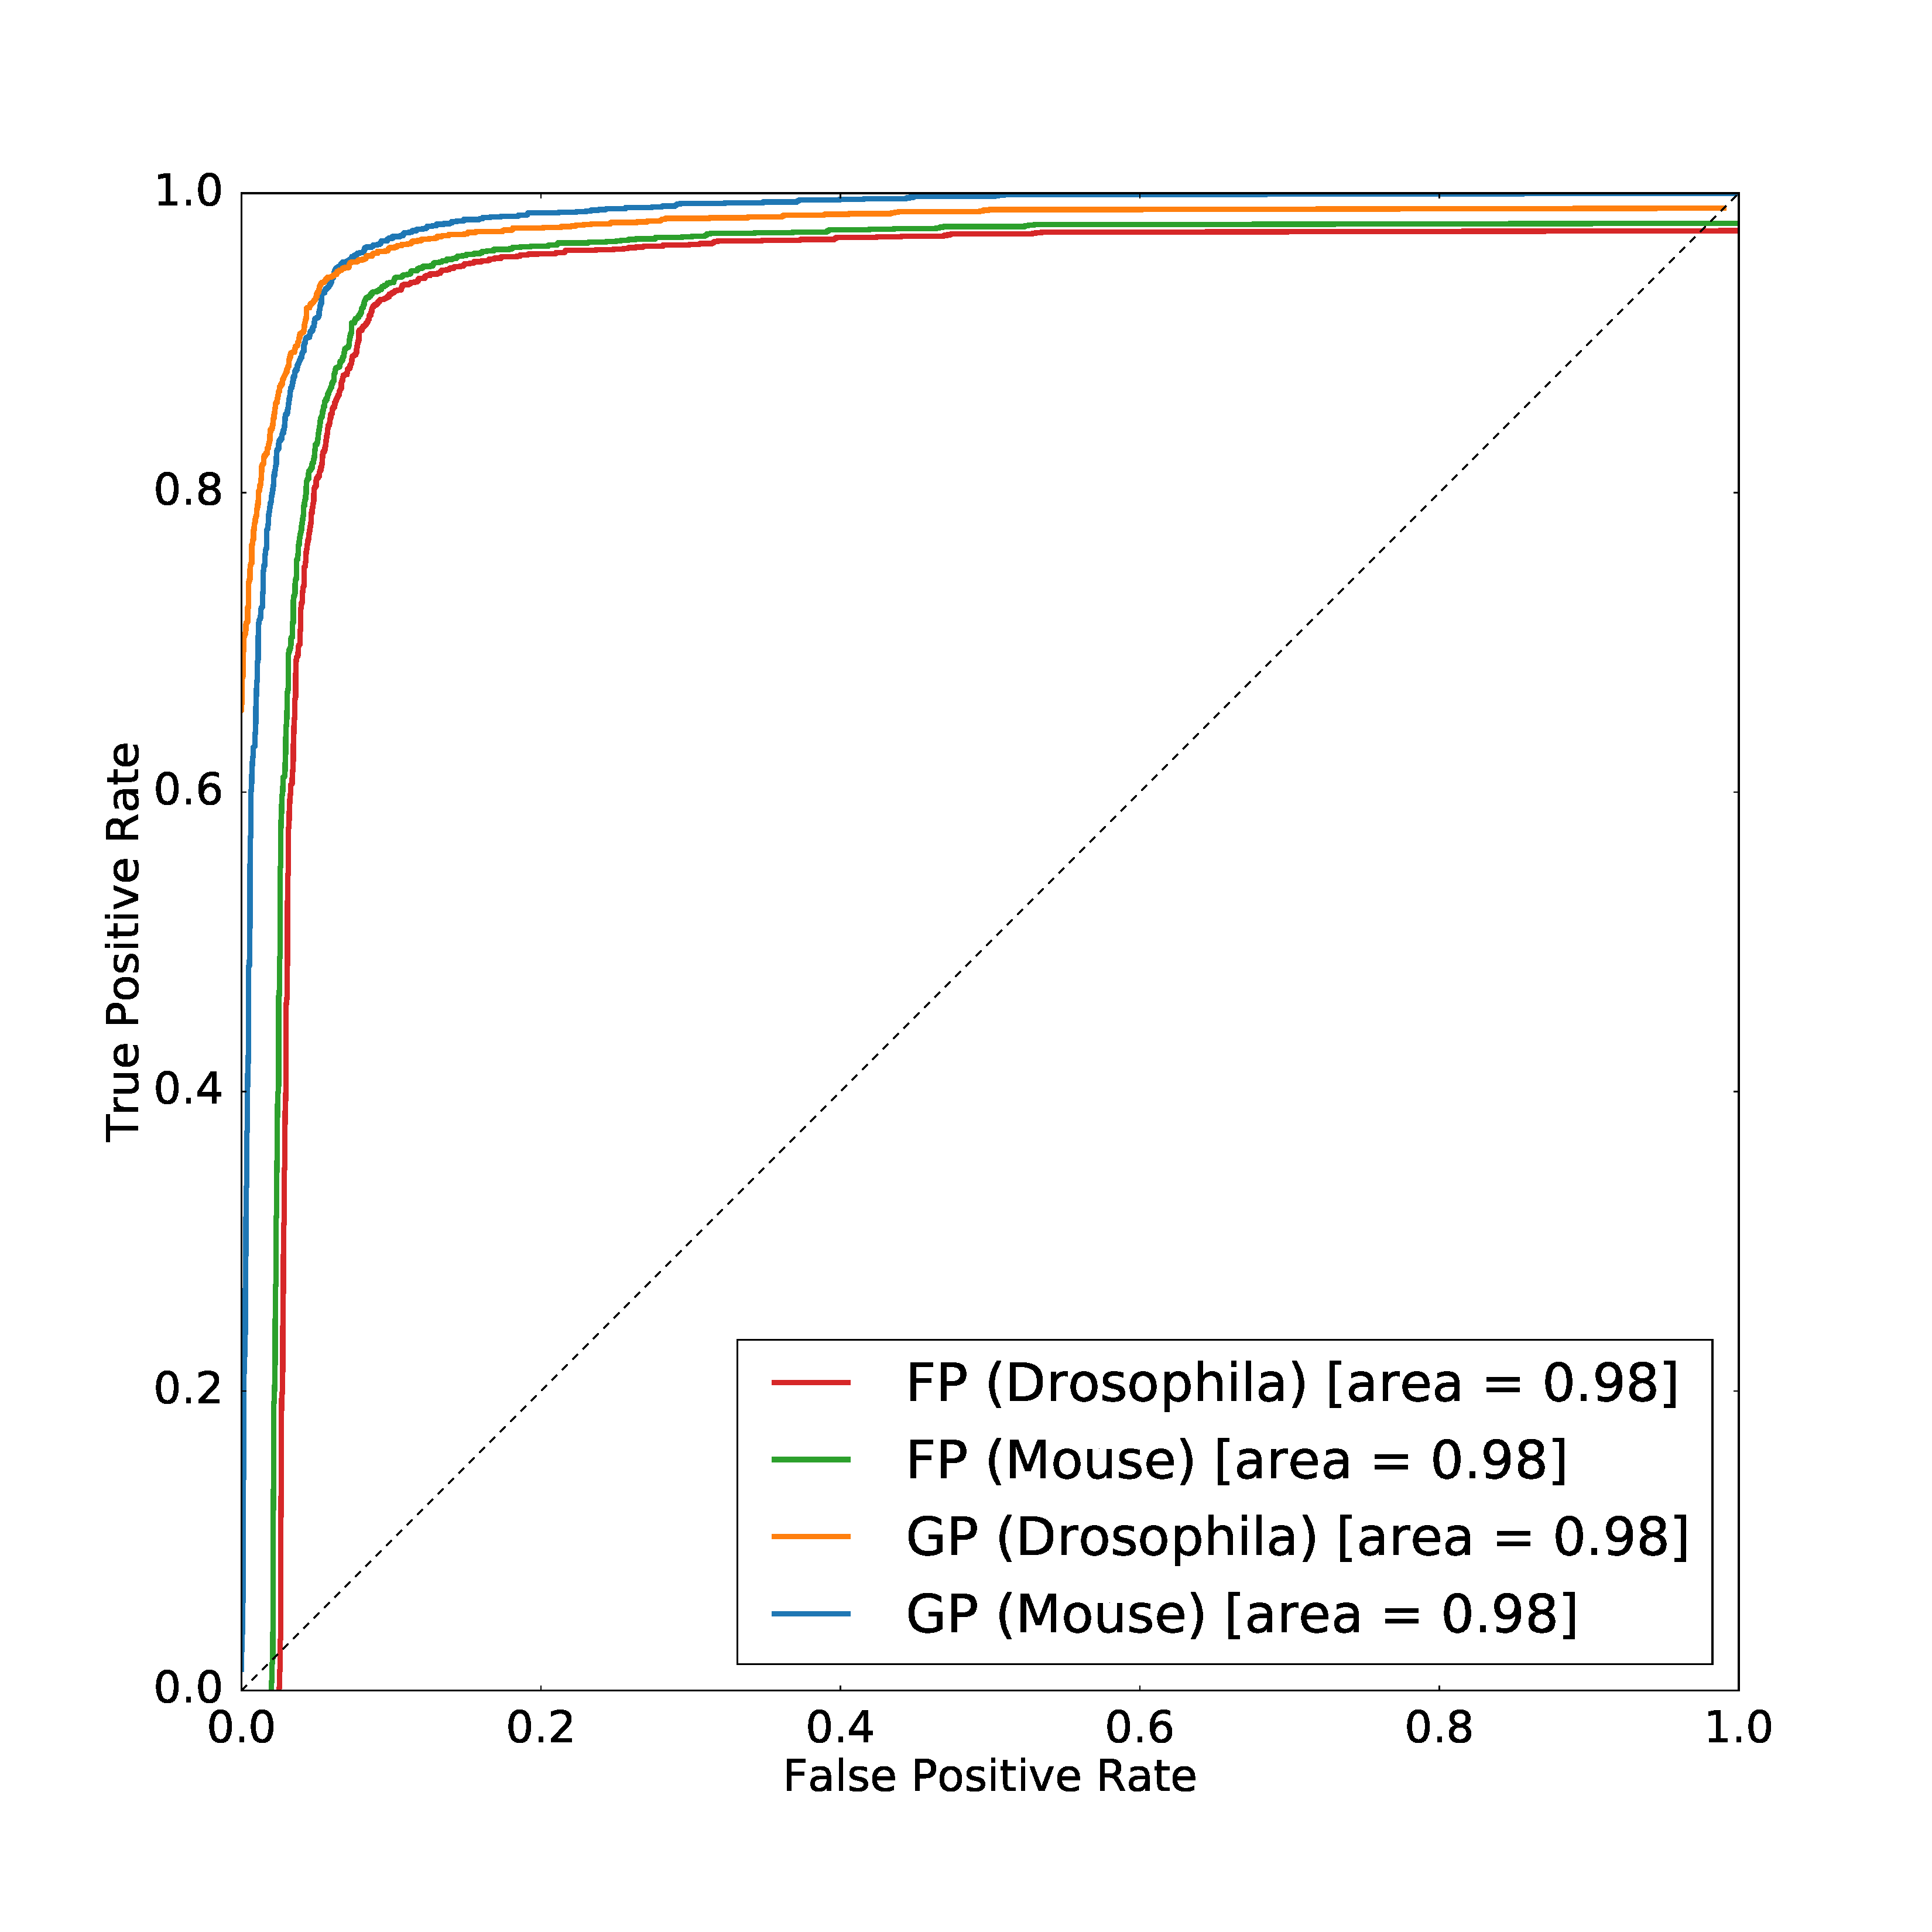
\includegraphics[width=\linewidth]{gfx/roc.pdf}
%\end{center}
%  \vspace{-10mm}
%   \caption{ROC performance of guided proofreading (GP) and focused proofreading (FP) trained separately on mouse and drosophila brain images. The area under the curve indicates better performance for GP.}
%\label{fig:roc}
%\end{figure}

%\subsection{Mouse Brain}
%
%Mouse brain is a common target for connectomics research because the structural proportions are similar to human brains~\cite{jeff_science}. For our first experiment we recruited novice and expert participants as part of a quantitative user study. Our second experiment is performed on a larger dataset and we evaluate a simulated user.
%\\~\\
%\textbf{User study.} Recently, Haehn \etal evaluated the interactive proofreading tools Raveler, Mojo, and Dojo as part of an experiment with novice users~\cite{haehn_dojo_2014}. The participants corrected an automatic segmentation with merge and split errors. The dataset was the most representative sub-volume (based on object size histograms) of a larger connectomics dataset and $400x400x10$ voxels in size. The participants were given a fixed time frame of 30 minutes to perform the correction interactively. While participants clearly struggled with the proofreading task, the best performing tool in their evaluation was Dojo. The dataset including manually labeled ground truth and the results of Haehn \etal are publicly available. This means we are able to use their findings as a baseline for comparison of GP for novices. In particular, we use the best performing user of Dojo who was truly an outlier as reported by Haehn \etal.
%
%Since interactive proofreading most likely yields lower performance than aided proofreading, we also compare against FP by Plaza~\cite{focused_proofreading} which is integrated in Raveler and freely available. For FP we consulted an expert to obtain the best possible parameters as shown in table \ref{tab:parameters}. Besides performance by novices, we are also interested in expert proofreading performance. Therefore, we design between-subjects experiments for 20 novice users and separately, for 6 expert users using the exact same conditions as Haehn \etal. The recruiting, consent and debriefing process is further described in the supplementary material. We randomly assign 10 novices to GP with active label suggestion (GP*) and 10 novices to FP. For the expert experiment, we assign accordingly.
%In addition to human performance, we also evaluate automatic GP, automatic GP with active label suggestion (GP*) and automatic FP. Due to the automatic nature, we do not enforce the 30 minute time limit but we stop once our probability threshold of $p_t=.95$ is reached. This value was observed as stable in previous experiments using automatic GP (see supplementary material). To measure proofreading performance in comparison to ground truth, we use the adapted Rand error (aRE) metric~\cite{RAND}. aRE is a measure of dissimilarity, related to introduced errors, meaning lower scores are better.
%
%The results of our comparisons are shown in the first row of Fig.~\ref{fig:results_mouse}. In all cases, GP* is able to correct the segmentation further than other methods (aRE measures: automatic GP XX, GP* XX, FP XX, novice Dojo XX, GP* XX, FP XX, expert Dojo XX, GP* XX, FP XX). This is not surprising since guided proofreading works for both merge and split errors while FP does not and in interactive Dojo the majority of time is spent finding errors which is minimized for aided proofreading solutions. In fact, the average correction time for novices is for GP* 3.6 (expert X), for FP Y (expert YY), and for Dojo 30 (expert ZZ) seconds.
%\\~\\
%\textbf{Simulated experiment.} For our second experiment with mouse brain data, we proofread the last 50 slices of the blue 3-cylinder mouse cortex volume of Kasthuri \etal~\cite{kasthuri2015saturated} which we also used for testing in section~\ref{sec:methods}. The data was not seen by the network before and includes $2048x2048x50$ voxels with a total number of 17,560 labeled objects. Since an interactive evaluation of such a large dataset would consume a significant amount of time, we restrict our experiment to a simulated (perfect) user and to automatic corrections, both with GP, GP* and FP. Similar to our comparison study, the simulated user assess a stream of errors by comparing the adapted Rand error measure before and after each performed correction. The simulated user is designed to be perfect and only accepts corrections if the measure is reduced. This time, we do not enforce a time limit to see the lower bound of possible corrections. For automatic GP and GP*, we use our defined probability threshold $p_t=.95$.
%
%The results of this experiment are shown in the second row of Fig.~\ref{fig:results_mouse}. GP* is again able to correct the segmentation further than other methods (aRE measures: automatic GP XX, GP* XX, FP XX, simulated GP* XX, FP XX). Again, the results are not surprising since GP* can correct merge and split errors.
%
%\subsection{Drosophila Brain}
%
%The drosophila brain is analyzed by connectomics researchers because of its small size and hence, a reasonable target to obtain a complete wiring diagram. Despite the size, fruit flies exhibit complex behaviors and are in general well studied. We evaluate the performance of our guided proofreading classifiers on three different datasets of adult fly brain. The datasets are publicly available as part of the MICCAI 2016 challenge on circuit reconstruction from electron microscopy images (CREMI)\footnote{The MICCAI CREMI challenge data is available at  http://www.cremi.org}. Each dataset consists of $1250x1250x125$ voxels of training data (A,B,C) as well as testing data (A+,B+,C+) of the same dimensions. Manually labeled ground truth is also available for A,B, and C but not for the testing data.
%
%Since drosophila brain exhibits different cell structures than mouse brain, we retrain the guided proofreading classifiers (and our automatic segmentation pipeline) as well as focused proofreading combined on the three training datasets. We use 300 slices of the A,B,C samples for training and validation, and 75 slices for testing. This results in YYY correct and ZZZ split error patches (respectively, XXX and YYY for testing). The architecture and all parameters of our classifiers stay the same. The trained GP classifier exhibits a reasonable performance on the testing data as seen in Fig.~\ref{fig:roc}.
%
%\begin{figure}[h]
%\begin{center}
%  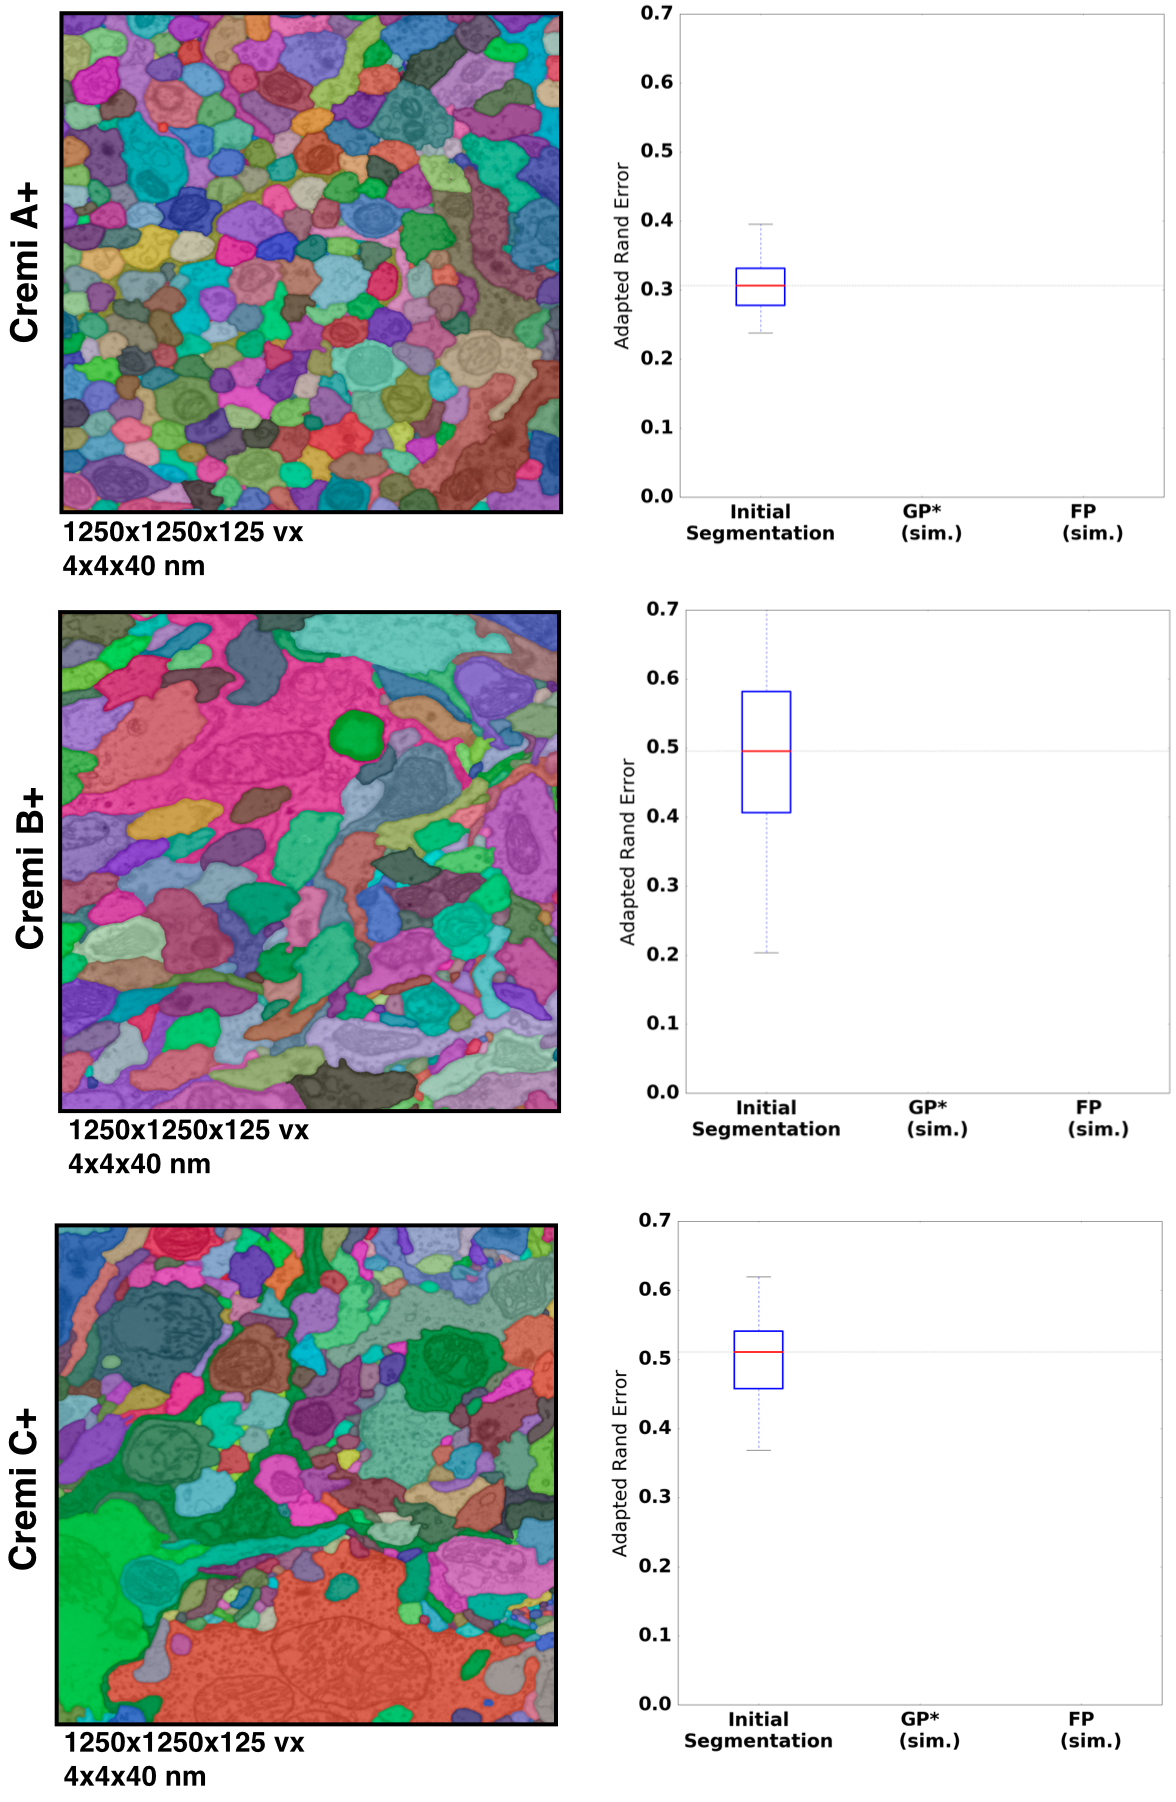
\includegraphics[width=\linewidth]{gfx/results_fruitfly.png}
%\end{center}
%  \vspace{-4mm}
%   \caption{Results of guided proofreading with active label suggestion (GP*) and focused proofreading performed automatically on three drosophila datasets. The datasets are part of the MICCAI 2016 CREMI challenge and publicly available. We measure performance as adapted Rand error (the lower, the better). GP* is able to correct the initial segmentation further than FP. Our GP* scores places us XXnd on the CREMI leaderboard.}
%\label{fig:results_fruitfly}
%\end{figure}
%
%We then use the trained GP* and FP classifiers to evaluate proofreading automatically. Since ground truth labeling is not available, the evaluation is performed by submitting our results to the CREMI leaderboard. Again, we use adapted Rand error to quantify the performance. Fig.~\ref{fig:results_fruitfly} shows the results for each of the A+,B+, and C+ datasets. The performance of GP* is significantly better than FP and places us XXnd on the CREMI leaderboard.
